\begin{table}[tbph]
          \begin{tabular}{@{\extracolsep{4pt}}l l r r r r r@{}}\hline
                    \multicolumn{2}{l}{Name} & \multicolumn{2}{c}{Initial Compile} & \multicolumn{2}{c}{Recompile} & Size \\
                    \cline{3-4}\cline{5-6}\cline{7-7}
                            & & KiB & ms & KiB & ms & KiB\\\hline
                    \hline\multicolumn{7}{l}{Hello, World}\\
                     & Dockerfile          &           748&     2,558&             0&       339&         1,086\\
                     & Squash and Load     &           748&     2,794&             0&       393&         1,086\\
                     & Layer Donning       &           748&     2,352&             0&       188&         1,086\\
                    \hline\multicolumn{7}{l}{Factorizer}\\
                     & Dockerfile a        &       119,067&     7,507&       116,719&     4,928&         5,343\\
                     & Dockerfile b        &       119,094&    11,207&             6&     1,540&        92,608\\
                     & Squash and Load     &       119,268&    10,552&       116,807&     8,306&         4,692\\
                     & Layer Donning       &        48,929&    18,754&             3&       782&         4,692\\
                    \hline\multicolumn{7}{l}{Blog}\\
                     & Dockerfile JS       &       431,817&   475,658&            73&    71,769&       473,635\\
                     & Dockerfile Go       &       430,215&   498,301&        68,845&   287,367&       473,635\\
                     & Squash and Load     &       433,128&   512,215&        68,965&   329,781&        12,700\\
                     & Layer Donning       &       410,628&   302,897&         3,089&    82,960&         8,736\\
                  \end{tabular}
                  \caption{Measurements}
                  \label{tab:measurements}
                \end{table}

                \def\diaghello--world{%
                  \pgfplotsset{enlargelimits=0.15,width=8cm,xticklabels={Dockerfile\\(Size: 1086 KiB),Squash and Load\\(Size: 1086 KiB),Layer Donning\\(Size: 1086 KiB)},xtick=data,ymin=0,tick label style={/pgf/number format/fixed,align=center}}\begin{figure}[htbp]
                    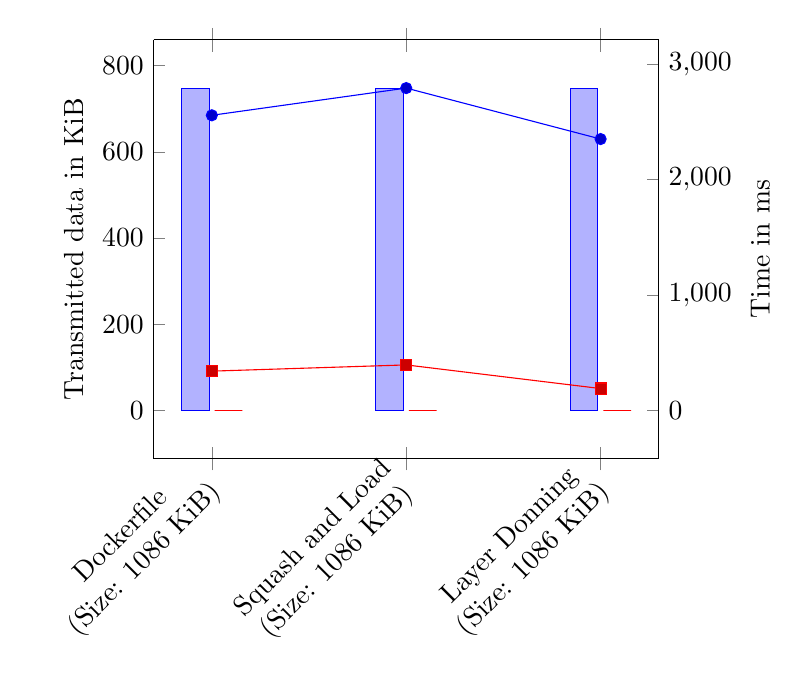
\begin{tikzpicture}
                      \begin{axis}[ybar,axis y line*=left,ylabel={Transmitted data in KiB},x tick label style={rotate=45,anchor=east},scaled y ticks = false]
                        \addplot coordinates {(0, 748) (1, 748) (2, 748) };\label{plot:hello--world-ttc-kib}
                        \addplot coordinates {(0, 0) (1, 0) (2, 0) };\label{plot:hello--world-ttrc-kib}
                      \end{axis}
                      \begin{axis}[axis y line*=right,ylabel={Time in ms},xticklabels={},scaled y ticks = false]
                        \addplot coordinates {(0, 2558) (1, 2794) (2, 2352) };\label{plot:hello--world-ttc-ms}
                        \addplot coordinates {(0, 339) (1, 393) (2, 188) };\label{plot:hello--world-ttrc-ms}
                      \end{axis}
                    \end{tikzpicture}
                    \caption{Measurement results for 'Hello, World' example}
                    \label{fig:mes-res-hello--world}
                  \end{figure}
                }

                \def\diagfactorizer{%
                  \pgfplotsset{enlargelimits=0.15,width=8cm,xticklabels={Dockerfile a\\(Size: 5343 KiB),Dockerfile b\\(Size: 92608 KiB),Squash and Load\\(Size: 4692 KiB),Layer Donning\\(Size: 4692 KiB)},xtick=data,ymin=0,tick label style={/pgf/number format/fixed,align=center}}\begin{figure}[htbp]
                    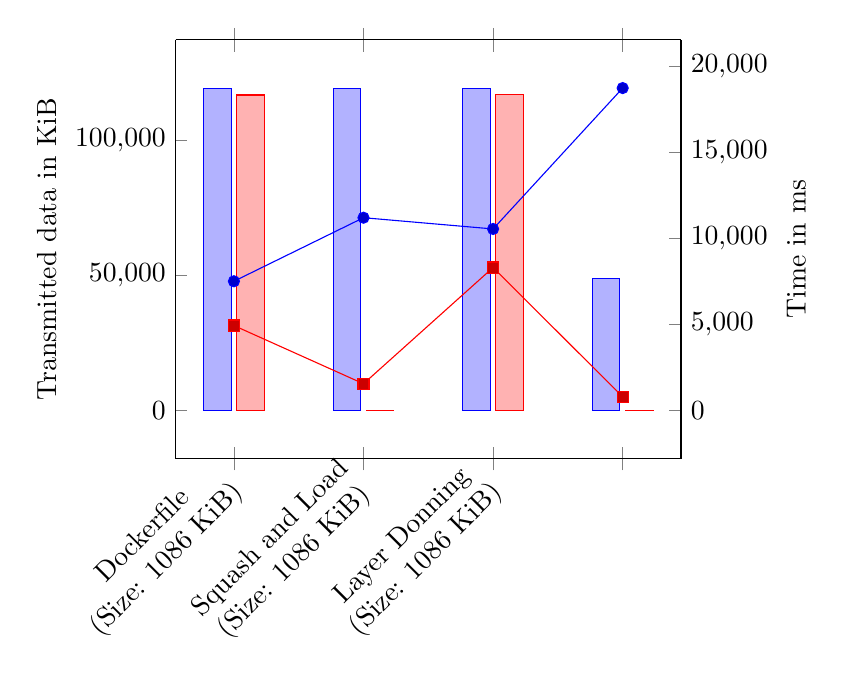
\begin{tikzpicture}
                      \begin{axis}[ybar,axis y line*=left,ylabel={Transmitted data in KiB},x tick label style={rotate=45,anchor=east},scaled y ticks = false]
                        \addplot coordinates {(0, 119067) (1, 119094) (2, 119268) (3, 48929) };\label{plot:factorizer-ttc-kib}
                        \addplot coordinates {(0, 116719) (1, 6) (2, 116807) (3, 3) };\label{plot:factorizer-ttrc-kib}
                      \end{axis}
                      \begin{axis}[axis y line*=right,ylabel={Time in ms},xticklabels={},scaled y ticks = false]
                        \addplot coordinates {(0, 7507) (1, 11207) (2, 10552) (3, 18754) };\label{plot:factorizer-ttc-ms}
                        \addplot coordinates {(0, 4928) (1, 1540) (2, 8306) (3, 782) };\label{plot:factorizer-ttrc-ms}
                      \end{axis}
                    \end{tikzpicture}
                    \caption{Measurement results for 'Factorizer' example}
                    \label{fig:mes-res-factorizer}
                  \end{figure}
                }


                \def\diagblog{%
                  \pgfplotsset{enlargelimits=0.15,width=8cm,xticklabels={Dockerfile JS\\(Size: 473635 KiB),Dockerfile Go\\(Size: 473635 KiB),Squash and Load\\(Size: 12700 KiB),Layer Donning\\(Size: 8736 KiB)},xtick=data,ymin=0,tick label style={/pgf/number format/fixed,align=center}}\begin{figure}[tbp]
                    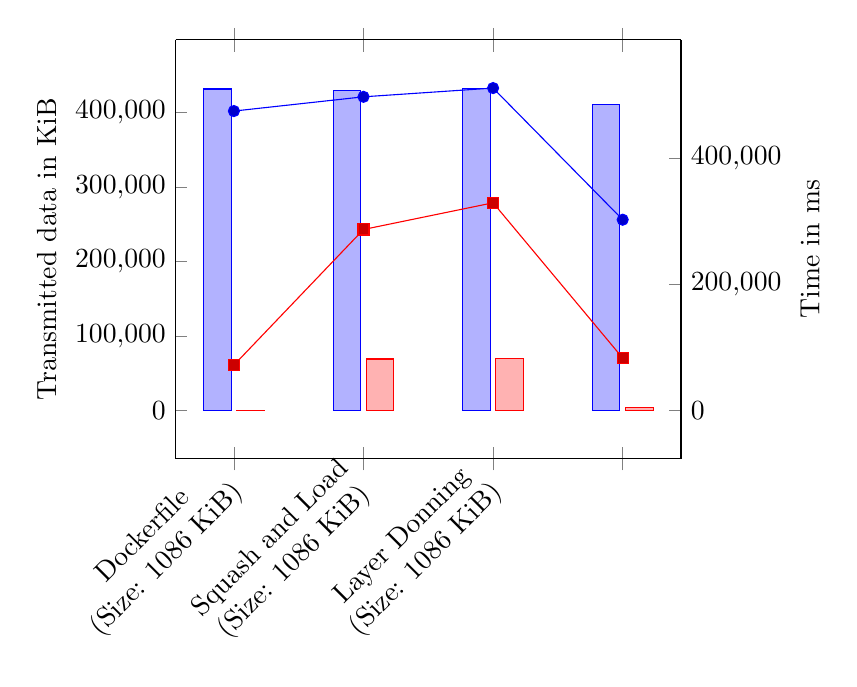
\begin{tikzpicture}
                      \begin{axis}[ybar,axis y line*=left,ylabel={Transmitted data in KiB},x tick label style={rotate=45,anchor=east},scaled y ticks = false]
                        \addplot coordinates {(0, 431817) (1, 430215) (2, 433128) (3, 410628) };\label{plot:blog-ttc-kib}
                        \addplot coordinates {(0, 73) (1, 68845) (2,  68965) (3, 3089) };\label{plot:blog-ttrc-kib}
                      \end{axis}
                      \begin{axis}[axis y line*=right,ylabel={Time in ms},xticklabels={},scaled y ticks = false]
                        \addplot coordinates {(0, 475658) (1, 498301) (2, 512215) (3, 302897) };\label{plot:blog-ttc-ms}
                        \addplot coordinates {(0, 71769) (1, 287367) (2, 329781) (3, 82960) };\label{plot:blog-ttrc-ms}
                      \end{axis}
                    \end{tikzpicture}
                    \caption{Measurement results for 'Blog' example}
                    \label{fig:mes-res-blog}
                  \end{figure}
                }
